\documentclass[a4paper,12pt]{article}
\usepackage[utf8]{inputenc}
\usepackage[T2A]{fontenc}
\usepackage[russian]{babel}
\usepackage{amsmath, amssymb}
\usepackage{graphicx}
\usepackage{booktabs}
\usepackage{hyperref}
\usepackage{caption}
\usepackage{float}

\begin{document}

\title{Предсказание волатильности российского фондового рынка: сравнительный анализ GARCH, LSTM и Transformer}
\author{Старченко Александр Николаевич\\
\small{Студент ИТМО}\\
\small{Email: astroblartvks@gmail.com}\\[5pt]
\small{Научный руководитель: Лабин Юрий Владимирович}}
\date{\today}
\maketitle

\begin{abstract}
В работе проведено сравнение классической эконометрической модели GARCH и нейросетевых архитектур LSTM и Transformer для задачи прогнозирования волатильности индекса Московской биржи (IMOEX). На дневных лог-доходностях за 2010--2026~гг. обучены модели, и оценена точность одношагового прогноза реализованной волатильности. Результаты показывают, что GARCH(1,1) превосходит обе нейросети по среднеквадратичной ошибке и коэффициенту детерминации \(R^2\), тогда как Transformer демонстрирует наихудшее качество. Обсуждаются причины неудачи Transformer на финансовых временных рядах и обозначены перспективы гибридного подхода GINN. 
\end{abstract}

\section{Введение}
Волатильность является одним из ключевых параметров в управлении финансовыми рисками. На её основе рассчитываются резервы капитала, стоимость опционов и величина VaR (Value-at-Risk). Точное предсказание волатильности особенно важно для развивающихся рынков, к которым относится и российский фондовый рынок. Индекс Мосбиржи (IMOEX) -- его основной индикатор; он подвержен резким скачкам, вызванным как глобальными шоками, так и внутренними событиями (кризисы 2014, 2020, 2022~гг.).

Классическим инструментом моделирования волатильности является семейство GARCH (Generalized Autoregressive Conditional Heteroskedasticity) \cite{Bollerslev1986}. Эти модели хорошо описывают кластеризацию волатильности, но могут плохо улавливать нелинейные зависимости. С развитием глубокого обучения для предсказания волатильности всё чаще применяются рекуррентные нейронные сети (LSTM, GRU) \cite{KimWon2018} и архитектуры на основе механизма внимания (Transformer) \cite{Vaswani2017}. Однако результаты сравнения неоднозначны: на одних рынках нейросети превосходят GARCH, на других -- уступают.

Для IMOEX уже проводилось сравнение GARCH и LSTM на данных до 2023~г. в выпускной квалификационной работе ВШЭ \cite{HSE_VKR}, где LSTM показал несколько лучшие результаты. Однако исследований с Transformer для российского индекса в открытом доступе не обнаружено. Более того, недавняя работа \cite{Xu2024} предложила гибридную архитектуру GINN (GARCH-Informed Neural Network), объединяющую GARCH и LSTM через специальную функцию потерь; модель показала преимущество на семи мировых индексах, но на российском рынке не тестировалась.

Цель данной работы -- провести прямое сравнение GARCH, LSTM и Transformer на данных IMOEX за максимально доступный период (2010--2026~гг.), оценить их способность предсказывать волатильность на один день вперёд и проанализировать поведение в кризисный период. Гибридная модель GINN исследуется отдельно и будет представлена в последующих публикациях.

\section{Обзор литературы}
Модель GARCH, предложенная Боллерслевом \cite{Bollerslev1986}, описывает условную дисперсию как линейную функцию прошлых квадратов ошибок и прошлых значений дисперсии. Для финансовых временных рядов чаще всего достаточно GARCH(1,1) \cite{HansenLunde2005}. Её преимущества -- интерпретируемость и малое число параметров; недостаток -- линейная структура, не учитывающая асимметрию и резкие смены режима.

Рекуррентные сети, особенно LSTM, активно применяются к предсказанию волатильности. Например, \cite{KimWon2018} использовали гибрид LSTM и GARCH для индекса KOSPI и показали улучшение точности. В работе \cite{HSE_VKR} на данных IMOEX~2013--2023 LSTM продемонстрировал лучшее качество по сравнению с GARCH, однако разница в периодах и методологии не позволяет напрямую обобщать результаты.

Transformer, первоначально разработанный для обработки естественного языка \cite{Vaswani2017}, был адаптирован для временных рядов. Его механизм самовнимания потенциально способен улавливать долгосрочные зависимости. Однако финансовые ряды обладают сильной локальной инерцией и редкими, но значимыми выбросами. Ряд исследований указывают на то, что Transformer без специальной модификации часто уступает LSTM в задачах с ограниченным объёмом данных \cite{Zeng2022}.

Гибридная модель GINN \cite{Xu2024} объединяет прогноз GARCH и нейросеть через выпуклую комбинацию в функции потерь: \( \mathcal{L} = \lambda\,\text{MSE}(\sigma^2_{\text{real}}, \hat{\sigma}^2_{\text{GINN}}) + (1-\lambda)\,\text{MSE}(\sigma^2_{\text{GARCH}}, \hat{\sigma}^2_{\text{GINN}}) \). При \(\lambda=0\) модель учится имитировать GARCH, что само по себе может давать более стабильный прогноз, чем обучение на реальной волатильности.

\section{Данные и описательная статистика}
Использовались ежедневные цены закрытия индекса IMOEX за период с 12.01.2010 по 03.04.2026 (4077 наблюдений), полученные с официального сайта Московской биржи. Дневные лог-доходности рассчитаны как
\begin{equation}
r_t = \ln\left(\frac{P_t}{P_{t-1}}\right) \times 100\%.
\end{equation}
Для них характерна кластеризация волатильности, «тяжёлые хвосты» и асимметрия (рис.~\ref{fig:returns}).

Реализованная волатильность (таргет) определялась как 20-дневное скользящее стандартное отклонение доходностей:
\begin{equation}
\sigma_t = \sqrt{\frac{1}{20}\sum_{i=0}^{19} (r_{t-i} - \bar{r}_t)^2}.
\end{equation}

Данные разделены на три непересекающихся периода:
\begin{itemize}
\item \textbf{Train}: 02.02.2010 -- 31.12.2019 (около 2500 дней);
\item \textbf{Validation}: 01.01.2020 -- 31.12.2021 (около 500 дней);
\item \textbf{Test}: 01.01.2022 -- 03.04.2026 (около 1062 дней).
\end{itemize}
Такое разбиение имитирует реальное применение: модель обучается на исторических данных, настраивается на «докризисном» 2020--2021 гг. и тестируется на новейшем периоде, включающем события 2022 года.

\begin{figure}[H]
\centering
\makebox[0pt][c]{%
  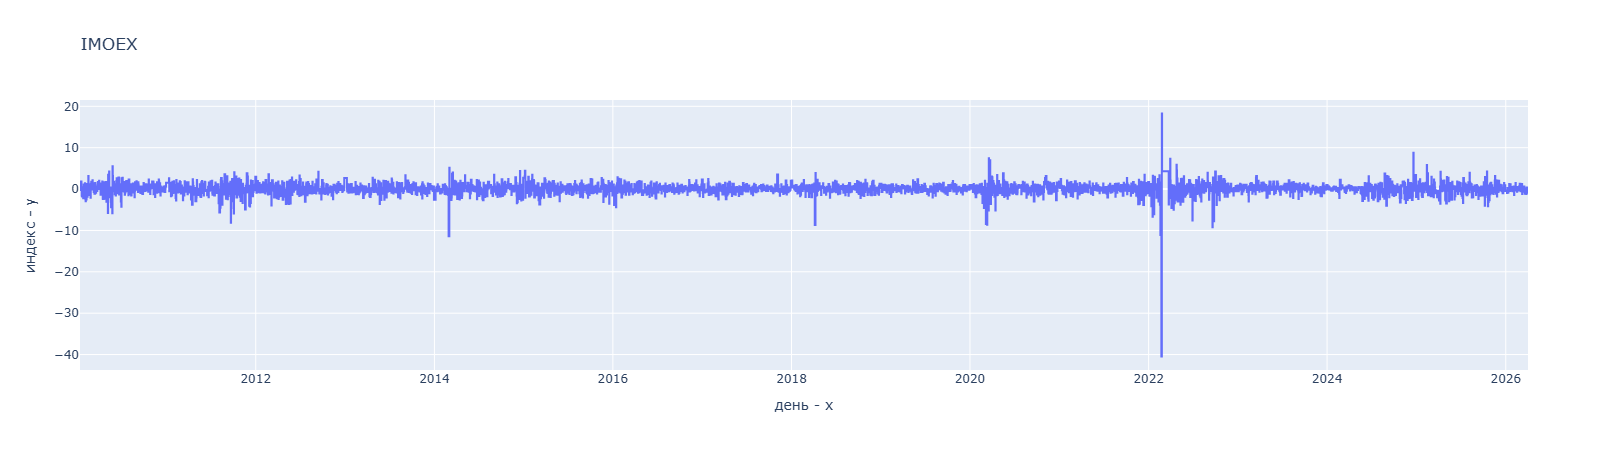
\includegraphics[width=0.85\paperwidth, height=0.35\textheight]{imoex_returns.png}%
}
\caption{Лог-доходности IMOEX (2010--2026).}
\label{fig:forecast_lstm}
\end{figure}

\section{Методология}

\subsection{GARCH(1,1)}
Модель задаётся уравнениями
\begin{align}
r_t &= \mu + \varepsilon_t,\\
\varepsilon_t &= \sigma_t z_t,\quad z_t \sim \mathcal{N}(0,1),\\
\sigma_t^2 &= \omega + \alpha \varepsilon_{t-1}^2 + \beta \sigma_{t-1}^2,
\end{align}
где \(\omega>0\), \(\alpha,\beta\ge 0\), \(\alpha+\beta<1\). Параметры оценивались методом максимального правдоподобия на окне длиной 90 дней. Для каждого дня тестовой выборки строился одношаговый прогноз дисперсии, из которого извлекался квадратный корень.

\subsection{LSTM}
Использовалась архитектура, аналогичная предложенной в \cite{Xu2024} для семейства GINN:
\begin{itemize}
\item Три слоя LSTM с 256 скрытыми нейронами каждый;
\item Dropout между слоями (0.2);
\item BatchNorm после последнего LSTM;
\item Два полносвязных слоя: 256 \(\to\) 128 (ReLU) \(\to\) 1.
\end{itemize}
Входной признак -- логарифм сглаженной реализованной дисперсии (методика \cite{Xu2024}):
\[
\sigma^2_t = \frac{1}{5}\sum_{i=0}^{4} (r_{t-i} - \hat{\mu}_{t-i})^2,
\]
где \(\hat{\mu}_t\) -- 90-дневное скользящее среднее. Применялось log-преобразование \(\ln(1+\sigma^2_t)\) для борьбы с тяжёлым правым хвостом. Модель обучалась предсказывать значение на следующий день по окну из 90 предыдущих значений. Обучение -- 300 эпох, оптимизатор AdamW с начальным шагом \(10^{-3}\) и уменьшением на плато. Ранняя остановка при отсутствии улучшения на валидации в течение 30 эпох. Функция потерь -- MSE.

\subsection{Transformer}
Реализован стандартный TransformerEncoder \cite{Vaswani2017}:
\begin{itemize}
\item Входной слой: линейное отображение 1 \(\to\) 64 (\(d_{model}=64\));
\item Позиционное кодирование (обучаемое);
\item 2 энкодерных слоя с 4 головами внимания и размером скрытого слоя 256;
\item Выходной слой: 64 \(\to\) 1 (ReLU, Dropout).
\end{itemize}
Обучение проводилось с теми же гиперпараметрами, что и LSTM, но потребовалось значительно меньше эпох до ранней остановки (78 эпох).

\subsection{Метрики}
Прогнозы денормализовывались (обратное log-преобразование) и сравнивались с \(\sigma_t\). Использовались:
\[
\text{MSE} = \frac{1}{N}\sum (\sigma_t - \hat{\sigma}_t)^2,\quad
\text{MAE} = \frac{1}{N}\sum |\sigma_t - \hat{\sigma}_t|,\quad
R^2 = 1 - \frac{\sum (\sigma_t - \hat{\sigma}_t)^2}{\sum (\sigma_t - \bar{\sigma})^2}.
\]

\section{Результаты}

\subsection{Сравнение точности прогнозов}
Основные результаты на тестовом периоде приведены в таблице~\ref{tab:metrics}. На рис.~\ref{fig:forecast} показаны прогнозы всех моделей вместе с реализованной волатильностью.

\begin{table}[H]
\centering
\caption{Метрики качества прогнозов на тестовой выборке (2022--2026).}
\label{tab:metrics}
\begin{tabular}{lccc}
\toprule
Модель & MSE & MAE & \(R^2\) \\
\midrule
GARCH(1,1) & 261.23 & 2.39 & 0.642 \\
LSTM       & 350.92 & 1.95 & 0.519 \\
Transformer & 635.62 & 2.45 & 0.128 \\
\bottomrule
\end{tabular}
\end{table}

GARCH оказался лидером по MSE и \(R^2\), объясняя около 64\% дисперсии реализованной волатильности. LSTM дал меньшую MAE, что говорит о меньшем среднем абсолютном отклонении, но хуже справился с выбросами. Transformer показал наихудшие результаты: \(R^2\) всего 0.13 свидетельствует о том, что модель практически не улавливает динамику волатильности.

\begin{figure}[H]
\centering
\makebox[0pt][c]{%
  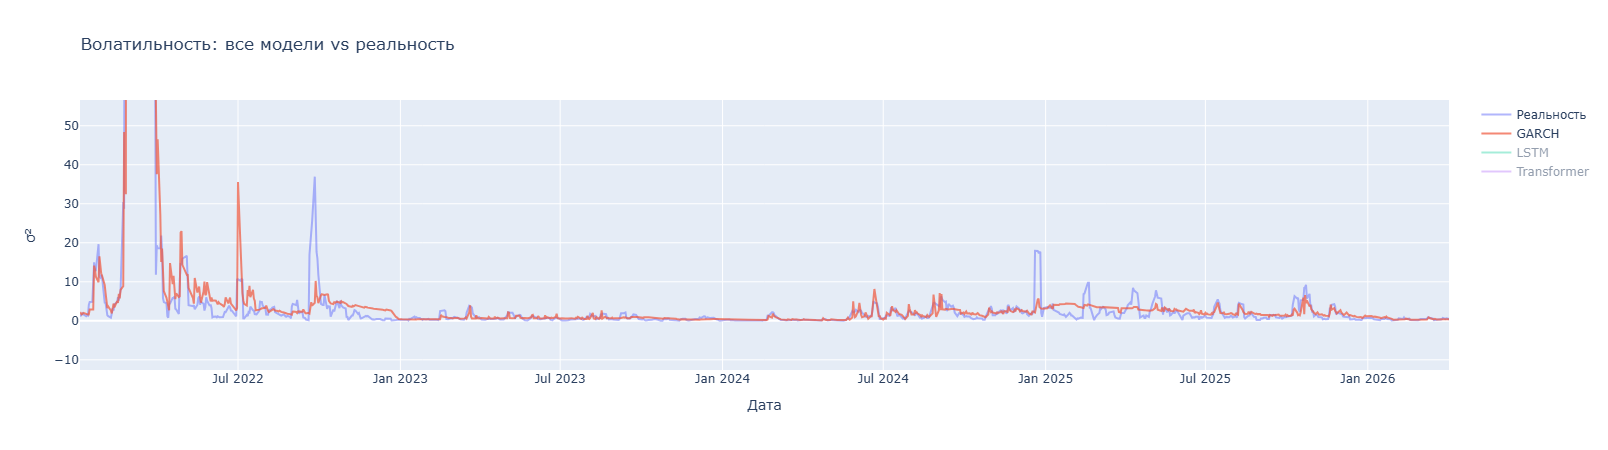
\includegraphics[width=0.82\paperwidth, height=0.35\textheight]{real_garch.png}%
}
\caption{Прогнозы GARCH на тестовом периоде (2022--2026).}
\label{fig:forecast_garch}
\end{figure}

\begin{figure}[H]
\centering
\makebox[0pt][c]{%
  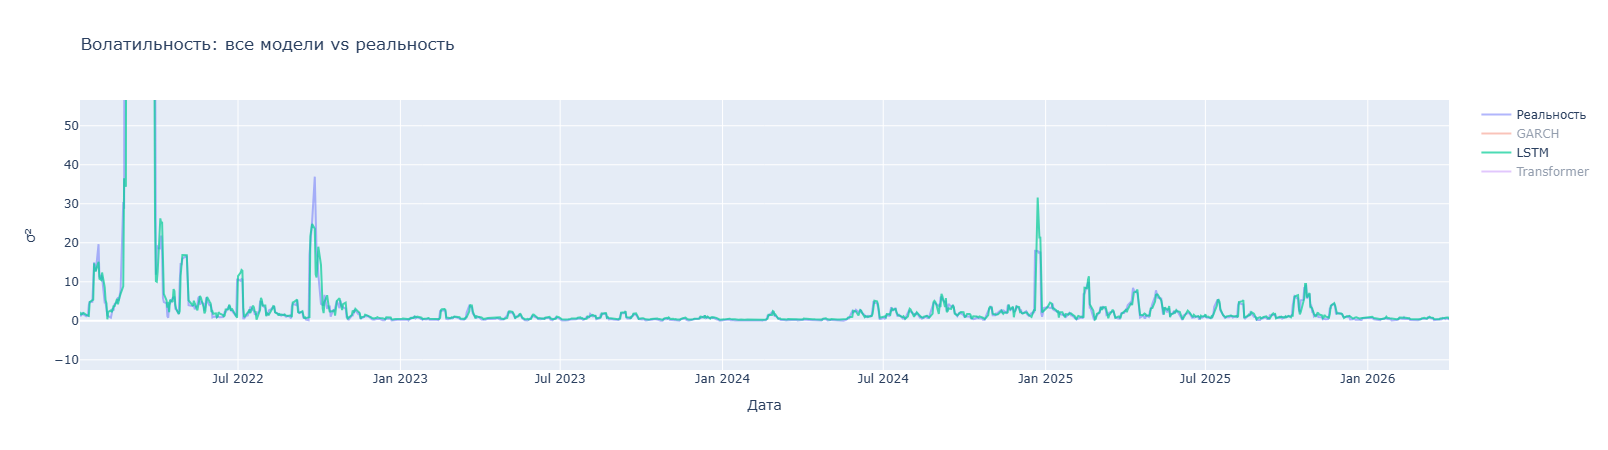
\includegraphics[width=0.82\paperwidth, height=0.35\textheight]{real_lstm.png}%
}
\caption{Прогнозы LSTM на тестовом периоде (2022--2026).}
\label{fig:forecast_lstm}
\end{figure}

\begin{figure}[H]
\centering
\makebox[0pt][c]{%
  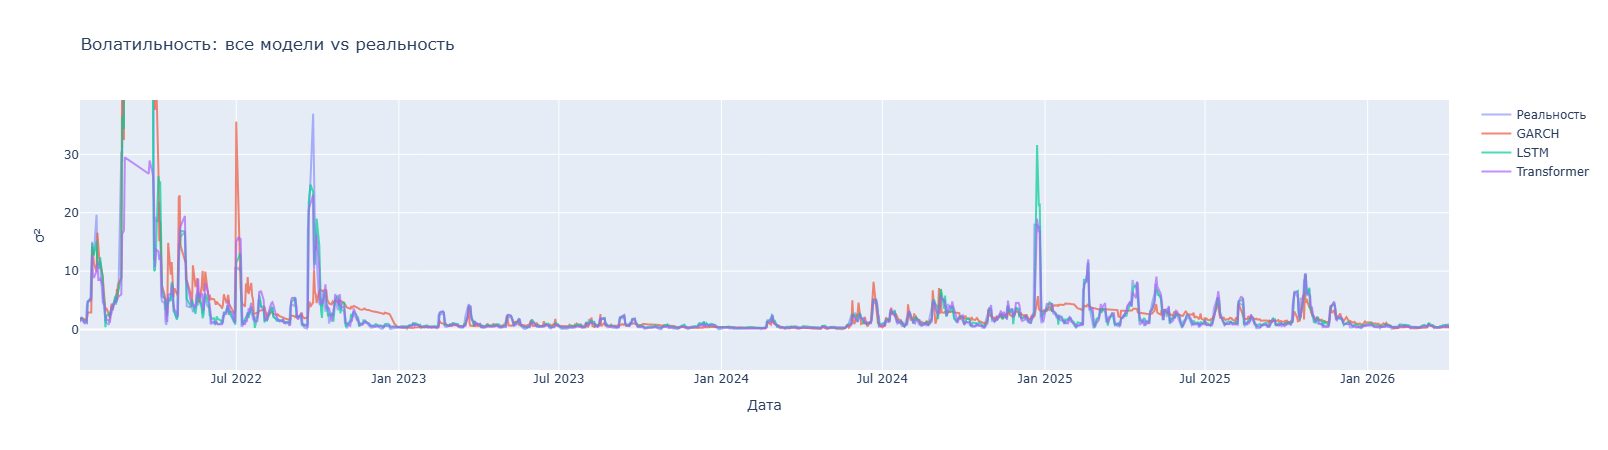
\includegraphics[width=0.82\paperwidth, height=0.35\textheight]{all_models_test.png}%
}
\caption{Прогнозы GARCH, LSTM и Transformer на тестовом периоде (2022--2026).}
\label{fig:forecast_all}
\end{figure}

\subsection{Поведение в кризисный период 2022 г.}
Наиболее яркий скачок волатильности пришёлся на конец февраля -- начало марта 2022 г. GARCH быстро отреагировал ростом прогнозной волатильности, хотя и с некоторым запаздыванием (рис.~\ref{fig:forecast_garch}). LSTM предсказал лишь умеренный рост, значительно недооценив масштаб шока (рис.~\ref{fig:forecast_lstm}). Transformer продемонстрировал почти плоскую линию, полностью проигнорировав всплеск (рис.~\ref{fig:forecast_all}). Это подтверждает известную проблему Transformer -- переобучение на спокойном режиме и неспособность к быстрой адаптации при смене режима без дополнительного дообучения.

\begin{figure}[H]
\centering
\makebox[0pt][c]{%
  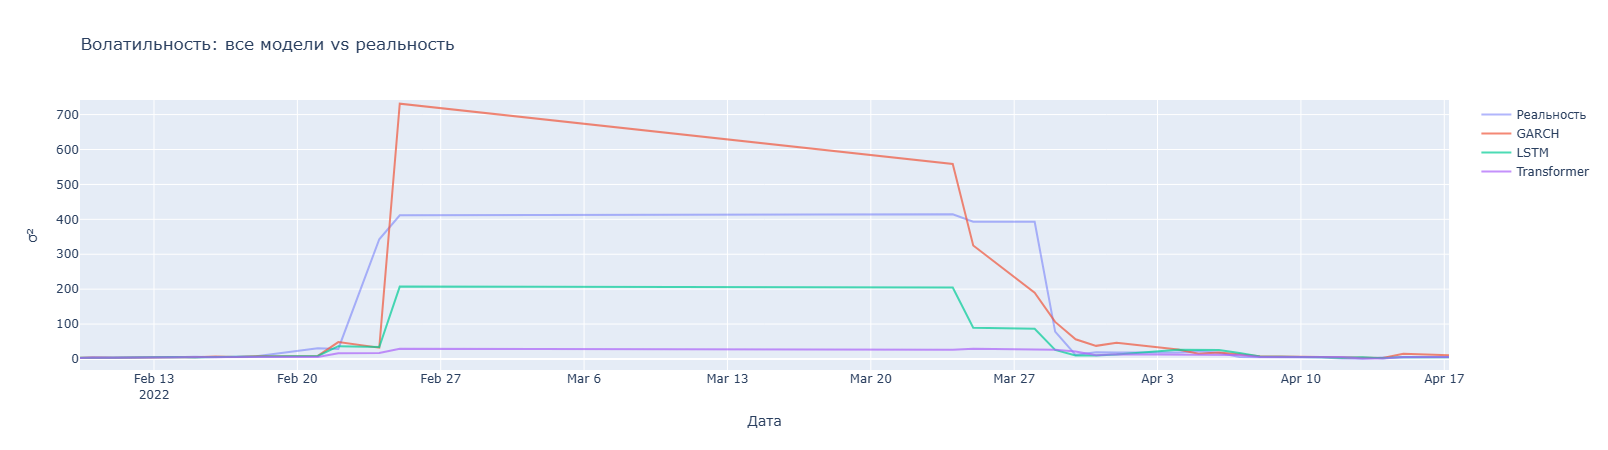
\includegraphics[width=0.82\paperwidth, height=0.35\textheight]{crisis_G_L_T.png}%
}
\caption{Кризис 2022 года: GARCH, LSTM и Transformer.}
\label{fig:crisis}
\end{figure}

\section{Обсуждение}
Уступая GARCH по MSE и \(R^2\), LSTM выигрывает по MAE, что может объясняться его способностью давать более гладкие прогнозы в спокойные периоды. Однако для риск-менеджмента важнее не промахнуться в хвостах, и здесь GARCH остаётся более надёжным инструментом.

Провал Transformer, на наш взгляд, обусловлен тремя причинами:
\begin{enumerate}
\item \textbf{Локальная структура данных}. Волатильность обладает сильной серийной зависимостью: сегодняшнее значение сильно коррелирует со вчерашним, но слабо -- с тем, что было 90 дней назад. Механизм самовнимания, ищущий глобальные взаимодействия, размывает эту локальную информацию.
\item \textbf{Недостаток данных}. Transformer'у требуется больше обучающих примеров, чем способен предоставить фондовый рынок (всего \(\sim\)2500 тренировочных окон).
\item \textbf{Переобучение на низкой волатильности}. Модель «запомнила» спокойный характер ряда, доминировавший в 2010-х, и экстраполирует его на любые будущие данные.
\end{enumerate}

Полученные результаты согласуются с выводами \cite{Xu2024} о том, что даже простой LSTM не всегда превосходит GARCH, и мотивируют развитие гибридных подходов, таких как GINN. Добавление GARCH-сигнала в функцию потерь может стабилизировать обучение нейросети и улучшить реакцию на стрессовые сценарии.

\section{Заключение}
В работе выполнено сравнение трёх моделей прогнозирования волатильности IMOEX. Классический GARCH(1,1) показал наилучшие результаты по точности, LSTM -- сопоставимое качество с меньшей MAE, а Transformer оказался непригоден для данной задачи в его стандартной реализации.

В дальнейшем планируется:
\begin{itemize}
\item Реализовать и исследовать гибридную модель GINN (включая вариант GINN-0) на российских данных;
\item Провести VaR-бэктестинг для оценки практической применимости моделей;
\item Включить в анализ кризисы 2014 и 2020 гг. путём расширения тестового периода или кросс-валидации.
\end{itemize}

\begin{thebibliography}{99}
\bibitem{Bollerslev1986} Bollerslev, T. (1986). Generalized autoregressive conditional heteroskedasticity. \textit{Journal of Econometrics}, 31(3), 307--327.
\bibitem{KimWon2018} Kim, H. Y., \& Won, C. H. (2018). Forecasting the volatility of stock price index: A hybrid model integrating LSTM with multiple GARCH-type models. \textit{Expert Systems with Applications}, 103, 25--37.
\bibitem{Vaswani2017} Vaswani, A. et al. (2017). Attention is all you need. \textit{Advances in Neural Information Processing Systems}, 30.
\bibitem{Xu2024} Xu, Q. et al. (2024). A GARCH-Informed Neural Network for Volatility Forecasting. \textit{Carnegie Mellon University / SSRN Working Paper}.
\bibitem{HSE_VKR} Выпускная квалификационная работа НИУ ВШЭ (2023). Прогнозирование волатильности российского фондового рынка с использованием LSTM и GARCH. URL: \url{https://www.hse.ru/edu/vkr/931805743}.
\bibitem{HansenLunde2005} Hansen, P. R., \& Lunde, A. (2005). A forecast comparison of volatility models: does anything beat a GARCH(1,1)? \textit{Journal of Applied Econometrics}, 20(7), 873--889.
\bibitem{Zeng2022} Zeng, A. et al. (2022). Are Transformers Effective for Time Series Forecasting? \textit{arXiv preprint arXiv:2205.13504}.
\end{thebibliography}

\end{document}